\documentclass[10pt]{article}
\usepackage[a4paper,margin=28mm]{geometry}
\usepackage[T1]{fontenc}
\usepackage{lmodern}
\usepackage{microtype}
\usepackage{amsmath,amssymb,amsthm}
\usepackage[colorlinks=true,linkcolor=blue!55!black,citecolor=blue!55!black,urlcolor=blue!55!black]{hyperref}
\usepackage{xcolor}
\usepackage{tikz}

\hypersetup{bookmarksnumbered=true}

\newtheorem{thm}{Theorem}[section]
\newtheorem{lem}[thm]{Lemma}
\newtheorem{cor}[thm]{Corollary}
\newtheorem*{claim*}{Claim}
\theoremstyle{remark}
\newtheorem{rmk}[thm]{Remark}

\newcommand{\calI}{\mathcal{I}}
\newcommand{\calP}{\mathcal{P}}

\title{The seven-cycle case of the maximal anti-Ramsey conjecture}
\author{Plasma AI}
\date{}

\begin{document}
\maketitle

\begin{abstract}
The maximal anti-Ramsey function $\chi_S(n,e,G)$ is the minimum number of colors needed to color the edges of some $n$-vertex, $e$-edge graph so that every copy of $G$ is rainbow. Burr, Erd\H{o}s, Graham and S\'{o}s conjectured that $\chi_S(n,\lfloor n^2/4\rfloor+1,C_{2k+1}) \sim n^2/8$ for every fixed $k\ge3$. Buci\'{c}, Chen and Ma proved it for $k\ge4$. We prove the remaining seven-cycle case, completing the proof of the conjecture. More generally, for $q=e/n^2$ we obtain
\[
 \chi_S(n,e,C_7)\ge
 \left(q-\frac18+\frac14\sqrt{q-\frac14}\right)n^2-o(n^2)
\]
uniformly over $\lfloor n^2/4\rfloor+1\le e\le\binom n2$. We also give a construction showing that the asymptotic formula for longer odd cycles fails for $C_7$ at every fixed density $1/4<q<1/2$.
\end{abstract}

\section{Introduction}

An edge-colored graph is \emph{rainbow} if all its edges have different colors. Classical anti-Ramsey theory began with Erd\H{o}s, Simonovits and S\'{o}s~\cite{ESS}, who studied how many colors force a rainbow copy of a fixed graph in an edge-coloring of $K_n$.

For a fixed graph $G$, the \emph{maximal anti-Ramsey function} $\chi_S(n,e,G)$, introduced and studied in~\cite{BEGS,BESFG}, is the minimum number of colors needed to color the edges of some $n$-vertex, $e$-edge graph so that every copy of $G$ is rainbow. Deleting edges shows that the same minimum is obtained if graphs with at least $e$ edges are allowed, as in~\cite{BCM}.

For connected bipartite $G$ that are not complete bipartite, S\'{a}rk\"{o}zy and Selkow~\cite[Theorem~4]{SS} proved that $\chi_S(n,e,G)/n\to\infty$ whenever $e/n^2$ stays bounded away from zero.

For odd cycles at $e=\lfloor n^2/4\rfloor+1$, the values of $\chi_S(n,e,C_3)$ and $\chi_S(n,e,C_5)$ are $3$ and $\lfloor n/2\rfloor+3$, respectively, for sufficiently large $n$. The latter result is due to Erd\H{o}s and Simonovits, as reported in~\cite[Sections~3--4]{BEGS}. For every fixed odd cycle of length at least seven, Burr, Erd\H{o}s, Graham and S\'{o}s~\cite[Theorem~5.1]{BEGS} proved a quadratic lower bound.

They conjectured that $\chi_S(n,\lfloor n^2/4\rfloor+1,C_{2k+1})\sim n^2/8$ for every fixed $k\ge3$~\cite[p.~270]{BEGS}. This is Erd\H{o}s Problem~809~\cite{Bloom809}. Buci\'{c}, Chen and Ma~\cite{BCM} proved the conjecture for $k\ge4$. We prove it for $k=3$.

\begin{thm}\label{thm:main}
As $n\to\infty$,
\[
  \chi_S\bigl(n,\lfloor n^2/4\rfloor+1,C_7\bigr)
       =\frac{n^2}{8}+o(n^2).
\]
\end{thm}

The upper bound was observed in~\cite{BEGS} (see also \cite[Section 2]{BCM}); it comes from the following construction. Take two disjoint cliques of nearly equal orders, color each injectively, and reuse the colors between the cliques. With a slight imbalance in their orders, one obtains the required number of edges. A modification using two cliques with one common vertex gives the sharper upper bound $n^2/8+O(n)$. We first prove the matching lower bound of $n^2/8-o(n^2)$ colors. We then use this threshold bound together with our weighted inequality to extend the lower bound to the full density range.

\begin{thm}\label{thm:density}
For $\lfloor n^2/4\rfloor+1\le e\le\binom n2$, put $q=e/n^2$. Then, as $n\to\infty$,
\begin{equation}\label{eq:densitybound}
 \chi_S(n,e,C_7)\ge
 \left(q-\frac18+\frac14\sqrt{q-\frac14}\right)n^2-o(n^2),
\end{equation}
where the error term is uniform in $e$.
\end{thm}

Buci\'{c}, Chen and Ma~\cite[Theorem~1.2]{BCM} determine the exact asymptotic coefficient for $C_{2k+1}$, $k\ge4$, throughout this range: it is $q/2+\frac12\sqrt{q-1/4}$. Writing $t=\sqrt{q-1/4}$, their coefficient exceeds the one in \eqref{eq:densitybound} by $t(1-2t)/4$, which is positive for $1/4<q<1/2$. Theorem~\ref{thm:density} gives a lower bound; we do not determine the exact asymptotic value at interior densities. At every fixed interior density, however, their formula fails for $C_7$.

\begin{thm}\label{thm:interior}
Fix $1/4<q<1/2$, and let $s\in(0,1/2)$ be the unique solution of
\[
 q=\frac12-3s^2+4s^3.
\]
Then, as $n\to\infty$,
\[
 \chi_S(n,\lfloor qn^2\rfloor,C_7)\le(q-s^3)n^2+O(n),
\]
and $q-s^3<q/2+\frac12\sqrt{q-1/4}$.
\end{thm}

For example, $q=3/8$ corresponds to $s=1/4$. At this density, Theorems~\ref{thm:density} and~\ref{thm:interior} give the lower and upper coefficients $(4+\sqrt2)/16\approx0.338$ and $23/64\approx0.359$, while the coefficient of~\cite{BCM} for longer odd cycles is $(3+2\sqrt2)/16\approx0.364$. We prove Theorem~\ref{thm:interior} in Section~\ref{sec:interior}, using a chain of five cliques.

For the lower bounds, we first study closed walks of length seven. Two edges joined by suitable walks of lengths two and three lie on such a walk. This observation leads to a weighted inequality in Sections~\ref{sec:clique} and~\ref{sec:finite}. A regularity argument then allows us to use it for cycles: after deleting at most $\eta n^2$ edges, no closed seven-walk contains two distinct edges of the same color (Corollary~\ref{cor:cleaning}). When $q$ stays bounded away from $1/4$, the cleaned graph still has density above $1/4$, and uniform vertex weights give Theorem~\ref{thm:density}.

Near the Tur\'{a}n threshold, these deletions may remove the single extra edge, while the weighted inequality requires density strictly greater than $1/4$. We separate graphs according to the variance of their normalized degrees $d(v)/n$. When this variance stays bounded away from zero, shifting a little weight toward vertices of above-average degree restores the required density. When the variance tends to zero, we can remove $o(n)$ vertices and obtain minimum degree $n/2-o(n)$ while preserving the edge excess. Section~\ref{sec:boundary} gives a direct color bound for these nearly regular graphs.

The arguments in Sections~\ref{sec:clique}--\ref{sec:finite}, \ref{sec:cleaning}, and \ref{sec:boundary} are independent of one another. Section~\ref{sec:assembly} combines the two variance cases to prove Theorem~\ref{thm:main}, then uses it to complete the density bound as $q$ approaches $1/4$.

Buci\'{c}, Chen and Ma~\cite[Sections~2 and~4]{BCM} use induction on $n$ to reduce to graphs of large minimum degree, where they construct large families of edges any two of which lie on a common $C_{2k+1}$. This requires the two short paths joining a pair of such edges to have total length at most $2k-1$, which for $k=3$ fails in their denser case, where $e/n^2$ is bounded away from $1/4$ and the paths can need $3+4$ edges. At the end of their proof they remark that a more involved ``stability'' argument, which they do not present, handles their near-threshold case for $k=3$, leaving the denser case as the main obstacle. Theorem~\ref{thm:interior} shows that this obstacle is genuine: their induction carries the bound of~\cite[Theorem~1.2]{BCM} through the whole range of $e$, and for $C_7$ that bound fails at every fixed interior density. Our proof does not use induction on $n$; apart from Section~\ref{sec:boundary}, which adapts short-path arguments from their near-threshold case to nearly regular graphs, it rests on the weighted inequality for closed seven-walks, fractional coloring, and regularity.

\paragraph{Formalization.} Theorem~\ref{thm:main} has been formalized in Lean~4 using Mathlib; the source code is available in~\cite{Formalization}.

\paragraph{Notation.} All graphs are finite and simple. Copies of graphs need not be induced. An $r$-walk or $r$-path has $r$ edges. A coloring is $C_7$-rainbow if every copy of $C_7$ is rainbow. We normalize edge density as $q=e/n^2$.

\section{A weighted bound for two- and three-walks}\label{sec:clique}

Suppose that edges $ab$ and $cd$ are joined by a two-edge walk from $a$ to $c$ and a three-edge walk from $b$ to $d$. Together they form a closed seven-walk containing both edges. We therefore seek large sets of vertices in which every pair can be joined by walks of both lengths.

Let $G$ be a graph, and let $A$ be its adjacency matrix. Let $w=(w_i)_i$ be a nonnegative column vector of vertex weights. Put
\[
 W=\mathbf1^{\mathsf T}w,\qquad d=Aw,\qquad
 Q=\frac12w^{\mathsf T}Aw,
\]
where $\mathbf1$ is the all-ones vector. Thus $d_i$ is the weighted degree of vertex $i$. For a vertex set $K$, write $w(K)=\sum_{i\in K}w_i$.

We introduce some terminology for the walk conditions that will recur in the proof. Note that $(A^r)_{ij}>0$ if and only if an $r$-edge walk in $G$ joins $i$ to $j$. Call a vertex $i$ \emph{triangular} if $(A^3)_{ii}>0$. A set $K$ is a \emph{joint clique} if $(A^2)_{ij}>0$ and $(A^3)_{ij}>0$ for every $i,j\in K$, including $i=j$. Thus every vertex of a joint clique is triangular. The next theorem shows that density above $W^2/4$ forces a joint clique containing more than half the total weight.

\begin{thm}\label{thm:joint}
Let $G$ and $w$ be as above. If every joint clique in $G$ has weight at most $s>0$, then
\begin{equation}\label{eq:jointcap}
 Q\le \frac{s^2+(W-s)^2}{2}.
\end{equation}
Consequently, if $Q>W^2/4$, some joint clique has weight at least
\begin{equation}\label{eq:jointroot}
 \frac W2+\sqrt{Q-\frac{W^2}{4}}.
\end{equation}
\end{thm}

We use the following weighted version of Hajnal's clique intersection lemma~\cite{Hajnal}. To apply it to joint cliques, form an auxiliary graph on the triangular vertices, joining distinct $i,j$ when both walk conditions hold. Its cliques are precisely the joint cliques.

\begin{lem}[Hajnal's lemma, weighted version]\label{lem:hajnal}
In a finite graph with nonnegative vertex weights, if $C_1,\ldots,C_r$ are maximum-weight cliques, each of weight $s$, then
\[
 w\Bigl(\bigcap_{j=1}^r C_j\Bigr)
 +w\Bigl(\bigcup_{j=1}^r C_j\Bigr)\ge 2s.
\]
\end{lem}
\begin{proof}
Let $I,U$ be the intersection and union of the first several cliques, and add a maximum clique $C$. The set $I\cup(C\cap U)$ is a clique, so $w(I\cup(C\cap U))=w(I\setminus C)+w(C\cap U)\le s=w(C)$. Thus $w(I\setminus C)\le w(C\setminus U)$, and it follows that $w(I\cap C)+w(U\cup C)\ge w(I)+w(U)$. The assertion follows by induction, starting with one clique, for which the sum is $2s$.
\end{proof}

\begin{proof}[Proof of Theorem~\ref{thm:joint}]
We prove \eqref{eq:jointcap} by optimizing over the vertex weights on $G$, with $s$ fixed. The admissible weights form the closed polyhedron
\[
 \calP_s=\{w\ge0:w(K)\le s\text{ for every joint clique }K\}.
\]
We will maximize the difference between the two sides of \eqref{eq:jointcap},
\[
 F_s(w)=Q-\frac{s^2+(W-s)^2}{2}
       =-\frac12w^{\mathsf T}(J-A)w+sW-s^2,
\]
where $J$ is the all-ones matrix.

Since $A_{ii}=0$ for every $i$, dropping nonpositive off-diagonal terms gives
\[
 F_s(w)\le -\frac12\sum_i w_i^2+s\sum_i w_i-s^2.
\]
The right-hand side tends to $-\infty$ as $\|w\|_2\to\infty$, so $F_s$ attains a global maximum on $\calP_s$. Suppose the maximum is positive, attained at $w\in\calP_s$. Set $u=W-s$. Since $Q\le W^2/2$, positivity implies $u>0$.

Since $A$ is symmetric,
\[
 \nabla F_s(w)=Aw-(W-s)\mathbf1=d-u\mathbf1.
\]
Decreasing a positive coordinate preserves feasibility. Its first-order condition is therefore
\begin{equation}\label{eq:degreewindowlow}
 d_i\ge u\qquad(w_i>0).
\end{equation}
We claim that $d_i\le s$ for every $i$. Otherwise take $p$ with $d_p>s$. If $w_i>0$ and $A_{pi}=1$, then $pi$ must be in a triangle of $G$. Indeed, if $N_G(p)\cap N_G(i)$ were empty, their weighted neighborhoods would be disjoint, so $d_i\le W-d_p<u$, contrary to \eqref{eq:degreewindowlow}. Now all positive-weight neighbors of $p$ form a joint clique: $a,p,b$ is a two-walk between any two of them, and if $c$ is the third vertex of a triangle containing $pa$, then $a,c,p,b$ is a three-walk. This works also when $a=b$. Its weight is $d_p>s$, a contradiction. Hence
\begin{equation}\label{eq:degreewindowhigh}
 d_i\le s\qquad\text{for all }i.
\end{equation}
In particular $2Q=w^{\mathsf T}d\le sW$. Positivity of $F_s(w)$ now gives $0<u<s$, and so $W<2s$.

Since $\calP_s$ is a polyhedron, the gradient at a maximizer is a nonnegative combination of the outward normals to its binding constraints. Thus there are multipliers $\mu_K\ge0$ for the clique constraints and $\nu_i\ge0$ for nonnegativity such that
\begin{equation}\label{eq:kkt}
 d_i-u=\sum_{K\ni i}\mu_K-\nu_i,\qquad
 \mu_K(w(K)-s)=0,\qquad \nu_iw_i=0.
\end{equation}
Put $L=\sum_K\mu_K$. Multiplying \eqref{eq:kkt} by $w_i$ and summing yields $2Q-uW=sL$. The strict inequality $F_s(w)>0$ implies
\[
 sL>s^2+u^2-u(s+u)=s(s-u),
\]
so $L>0$. All cliques with $\mu_K>0$ have weight $s$ and are therefore maximum-weight joint cliques. Lemma~\ref{lem:hajnal} says that their intersection has weight at least $2s-W=s-u>0$. Choose a positive-weight vertex $p$ in that intersection. Equation~\eqref{eq:kkt} gives $d_p-u=L>s-u$, contradicting \eqref{eq:degreewindowhigh}. This proves \eqref{eq:jointcap}.

Let $M$ be the maximum joint-clique weight when $Q>W^2/4$. Equation~\eqref{eq:jointcap} with $s=W/2$ shows $M>W/2$. Apply it again with $s=M$ and solve the resulting quadratic inequality on the interval $M>W/2$ to obtain \eqref{eq:jointroot}.
\end{proof}

\begin{rmk}
The bounds in Theorem~\ref{thm:joint} are asymptotically sharp. Fix $W>0$ and $W/2\le M\le W$. For each integer $t\ge3$, take two disjoint copies of $K_t$, with vertex weights $M/t$ in one and $(W-M)/t$ in the other. The largest joint clique has weight $M$, and
\[
 Q=\left(1-\frac1t\right)\frac{M^2+(W-M)^2}{2}.
\]
As $t\to\infty$, this approaches the bound in \eqref{eq:jointcap} with $s=M$. If $M>W/2$, then $Q>W^2/4$ for all sufficiently large $t$, and the lower bound in \eqref{eq:jointroot} tends to $M$.
\end{rmk}

\section{Fractional colorings and the seven-cycle inequality}\label{sec:finite}

We continue in the setting of Section~\ref{sec:clique}. Assume that $\sum_iw_i=1$. To each edge $ij$ of $G$, assign the weight $w_iw_j$. Then
\[
Q=\sum_{ij\in E(G)}w_iw_j.
\]
Define a \emph{conflict graph} $J_{23}=J_{23}(G)$ with vertex set $E(G)$ by joining two edges if they admit orientations $(a,b)$ and $(c,d)$ for which
\begin{equation}\label{eq:conflict}
 (A^2)_{ac}>0\quad\text{and}\quad(A^3)_{bd}>0.
\end{equation}
The two walks implied by \eqref{eq:conflict}, together with $ab$ and $cd$, form a closed seven-walk. Consequently, if no closed seven-walk contains two distinct edges of the same color, each color class is an independent set of $J_{23}$. Corollary~\ref{cor:cleaning} shows how to achieve this condition by deleting a small number of edges when every $C_7$ is rainbow.

To account for these edge weights, we use fractional colorings. For a finite simple graph $\Gamma$, let $\calI(\Gamma)$ be its nonempty independent sets; vertices in one such set may share a color. Given nonnegative numbers $d_i$ specifying the required coverage of each vertex, define the fractional coloring cost by
\begin{equation}\label{eq:phi}
 \Phi(\Gamma;d)=\min\left\{\sum_{I\in\calI(\Gamma)}z_I:
 z_I\ge0,\quad\sum_{I\ni i}z_I\ge d_i\ (\forall i)\right\}.
\end{equation}
Finite linear programming duality gives
\begin{equation}\label{eq:phidual}
 \Phi(\Gamma;d)=\max\left\{\sum_i d_iy_i:y_i\ge0,
 \quad\sum_{i\in I}y_i\le1\ (\forall I\in\calI(\Gamma))\right\}.
\end{equation}
Call an allocation $z$ \emph{exact} if $\sum_{I\ni i}z_I=d_i$ for every $i$. Any optimum in \eqref{eq:phi} can be made exact: when a vertex receives more than $d_i$, split weights $z_I$ as needed and remove the vertex from some of the corresponding independent sets. Discard empty sets; the total cost does not increase.

Using only singleton independent sets costs $\sum_i d_i$. The next lemma bounds the saving from using larger independent sets, with a stronger bound when a clique contains at least half the vertex weight.

\begin{lem}[Fractional coloring savings]\label{lem:palette}
Let $v_i\ge0$ sum to one and let $\alpha_i\ge0$ be feasible in \eqref{eq:phidual}. With $R=\Phi(\Gamma;(v_i\alpha_i)_i)$,
\begin{equation}\label{eq:savequarter}
 \sum_i v_i\alpha_i-R\le\frac14.
\end{equation}
If $\Gamma$ contains a clique of $v$-mass $p\ge1/2$, then
\begin{equation}\label{eq:saveclique}
 \sum_i v_i\alpha_i-R\le p(1-p).
\end{equation}
\end{lem}
\begin{proof}
The dual vector $y_i=\alpha_i$ gives $R\ge\sum_i v_i\alpha_i^2$. Singleton sets give $0\le\alpha_i\le1$, and $a(1-a)\le1/4$ proves \eqref{eq:savequarter}.

For \eqref{eq:saveclique}, let $L$ be the clique and take an exact optimal allocation $z_I$. Exact coverage expresses the saving as $\sum_I(|I|-1)z_I$. We seek coefficients $c_i$ such that $\sum_{i\in I}c_i\ge |I|-1$ whenever $z_I>0$; multiplying by $z_I$ and summing will then bound the saving by $\sum_{i:\alpha_i>0}c_iv_i\alpha_i$. If $z_I>0$, exact coverage gives $v_i\alpha_i>0$ for every $i\in I$, so $\alpha_i>0$. For these vertices, set
\[
 c_i=\begin{cases}(1-p)^2/\alpha_i,&i\in L,\\
                   p^2/\alpha_i,&i\notin L.
       \end{cases}
\]
Every independent set $I$ with $z_I>0$ satisfies $\sum_{i\in I}c_i\ge |I|-1$. Indeed, it contains at most one vertex of $L$. If it contains one with value $a$ and $k\ge1$ others with values $b_j$, Cauchy--Schwarz and dual feasibility give
\[
 \frac{(1-p)^2}{a}+p^2\sum_{j=1}^k\frac1{b_j}
 \ge\frac{(1-p+pk)^2}{a+\sum_jb_j}
 \ge(1-p+pk)^2\ge k.
\]
The last step uses $p\ge1/2$ and $k\ge1$; the case $k=0$ is immediate. If $I$ avoids $L$ and has $k\ge1$ vertices, then $p^2\sum_{i\in I}1/\alpha_i\ge p^2k^2\ge k-1$. Exact coverage therefore yields
\[
 \begin{aligned}
 \sum_i v_i\alpha_i-R
 &=\sum_I(|I|-1)z_I
 \le\sum_{i:\alpha_i>0} c_iv_i\alpha_i\\
 &\le (1-p)^2p+p^2(1-p)=p(1-p).
 \end{aligned}
\]
\end{proof}

We apply this estimate to the conflict graph, with the edge weights $w_iw_j$ as the required coverages. If no closed seven-walk repeats a color on distinct edges, each color class is independent in $J_{23}$. With uniform vertex weights $1/n$, assigning each nonempty such class weight $1/n^2$ therefore shows that the fractional coloring cost $C$ below is at most $r/n^2$, where $r$ is the number of colors.

\begin{thm}\label{thm:finite}
Let $G$ be a graph with nonnegative vertex weights $w$ summing to $1$, and put
\[
 Q=\sum_{ij\in E(G)}w_iw_j,\qquad C=\Phi(J_{23}(G);(w_iw_j)_{ij\in E(G)}).
\]
If $Q>1/4$, then
\begin{equation}\label{eq:finitebound}
 C\ge Q-\frac18+\frac14\sqrt{Q-\frac14}>\frac18.
\end{equation}
\end{thm}
\begin{proof}
Choose a joint clique $K$ of mass $m=w(K)\ge\frac12+\sqrt{Q-1/4}$ by Theorem~\ref{thm:joint}. Write $U=V(G)\setminus K$, $u=w(U)=1-m$, and let $Q_K,Q_{KU},Q_U$ be the edge masses inside $K$, across $(K,U)$, and inside $U$, respectively. Thus $Q=Q_K+Q_{KU}+Q_U$. We will show that $Q-C\le u/4$; the lower bound on $m$ will then give \eqref{eq:finitebound}.

Edges within $K$ form a clique in $J_{23}$, and each conflicts with every edge crossing from $K$ to $U$. For the latter assertion, the two-walk joins their $K$ endpoints, while a two-walk between vertices of $K$ followed by the crossing edge gives the three-walk required in \eqref{eq:conflict}. Consequently, if $C_{\rm cut}$ denotes the fractional coloring cost of the crossing edges, duality gives $C\ge Q_K+C_{\rm cut}$. If $u=0$, this says $C=Q$; suppose $u>0$.

Define a graph $\Gamma$ on $U$ by joining distinct $x,y$ whenever a two- \emph{or} a three-walk joins them in $G$. Put
\[
 g_x=\sum_{i\in K}w_iA_{ix},\qquad \rho_x=w_xg_x,
 \qquad Q_{KU}=\sum_{x\in U}\rho_x.
\]
An independent set of crossing edges in $J_{23}$ has distinct outside endpoints, and these endpoints form an independent set in $\Gamma$. Two edges with the same outside endpoint conflict by a closed two-walk there and a three-walk between their $K$ endpoints. If two different outside endpoints admit a two-walk, use the three-walk between $K$ endpoints; if they admit a three-walk, use the two-walk between $K$ endpoints. Project an exact allocation for the crossing edges to their outside endpoints. It covers $\rho_x$ exactly, whence, with $R=\Phi(\Gamma;\rho)$,
\begin{equation}\label{eq:cutreduction}
 C\ge Q_K+R,\qquad Q-C\le Q_U+Q_{KU}-R.
\end{equation}

For any independent set $I$ of $\Gamma$, the neighborhoods $N_G(x)\cap K$, $x\in I$, are pairwise disjoint: a common neighbor would give a two-walk. Hence $\sum_{x\in I}g_x\le m$. Set $v_x=w_x/u$ and $\alpha_x=g_x/m$. The vector $\alpha$ is dual feasible, and $\rho_x=mu\,v_x\alpha_x$. Lemma~\ref{lem:palette} and homogeneity give
\begin{equation}\label{eq:crosssave}
 Q_{KU}-R\le\frac{mu}{4}.
\end{equation}
If $\Gamma$ has a clique $L$ of original weight $\ell\ge u/2$, the stronger conclusion is
\begin{equation}\label{eq:crosssaveclique}
 Q_{KU}-R\le\frac m u\,\ell(u-\ell).
\end{equation}

To finish, compare the edge mass $Q_U$ inside $U$ with $u^2/4$. If $Q_U\le u^2/4$, equations \eqref{eq:cutreduction} and \eqref{eq:crosssave} give $Q-C\le Q_U+mu/4\le(u^2+mu)/4=u/4$.

If $Q_U>u^2/4$, Theorem~\ref{thm:joint} yields a joint clique within $U$, allowing us to use the stronger savings bound. Its weight satisfies $\ell\ge u/2+\sqrt{Q_U-u^2/4}$. Its walks in $G[U]$ are also walks in $G$, so it is a clique of $\Gamma$, and
\[
 \ell(u-\ell)\le\frac{u^2}{2}-Q_U.
\]
Since $m\ge u$, equations \eqref{eq:cutreduction} and \eqref{eq:crosssaveclique} imply
\[
 Q-C\le Q_U+\frac m u\ell(u-\ell)
 \le\frac{mu}{2}+\Bigl(1-\frac m u\Bigr)Q_U
 \le\frac{mu+u^2}{4}=\frac u4.
\]
Thus always $C\ge Q-(1-m)/4$. Inserting the lower bound on $m$ proves \eqref{eq:finitebound}.
\end{proof}

\section{From closed walks to cycles}\label{sec:cleaning}

We use Szemer\'{e}di's regularity lemma~\cite{Szemeredi} and the embedding lemma of Koml\'{o}s and Simonovits~\cite[Theorem~2.1]{KS} to pass from closed walks to cycles. The point needed here is that two specified edges can be kept fixed.

\begin{lem}[Seven-walk cleaning]\label{lem:cleaning}
For every $\eta>0$, if $n$ is sufficiently large, then every $n$-vertex simple graph $G$ has a spanning subgraph $H\subseteq G$, obtained by deleting at most $\eta n^2$ edges, such that any two distinct edges belonging to a common closed seven-walk in $H$ belong to a common $C_7$ in $G$.
\end{lem}

\begin{proof}
Choose $0<d<1$ small in terms of $\eta$, then a large integer $t_0$, and finally $\varepsilon>0$ small in terms of $d$ and $\eta$. Apply the equitable regularity lemma to partition $V(G)$ into an exceptional set of size at most $\varepsilon n$ and $t\ge t_0$ equal-sized parts, each of size $M$. At most $\varepsilon t^2$ pairs of parts are irregular. Delete edges meeting the exceptional set, edges within parts, edges in irregular pairs, and edges in pairs of density below $d$.

We also trim vertices with unusually small degree in a retained pair. In a pair of original density $p$, delete the edges of that pair incident to any vertex with fewer than $(p-\varepsilon)M$ neighbors in the opposite part. Regularity bounds the number of such vertices by $\varepsilon M$ on each side. The total deletion cost is $O(d+\varepsilon+t_0^{-1})n^2<\eta n^2$. Denote the remaining graph by $H$.

\begin{claim*}
      A walk $x_0,\ldots,x_r$ in $H$ with distinct endpoints and $3\le r\le5$ can be replaced by a path in $G$ with the same endpoints, length and sequence of parts. The path can also avoid any set of at most three vertices other than its endpoints.
\end{claim*}
\begin{proof}[Proof of the claim]
      Let $V_j$ be the part containing $x_j$. Set $S_1=N_G(x_0)\cap V_1$, $S_{r-1}=N_G(x_r)\cap V_{r-1}$, and $S_j=V_j$ for $2\le j\le r-2$. Trimming gives $|S_j|\ge(d-\varepsilon)M$ for every $j$. After removing $x_0,x_r$ and the forbidden vertices, each set still has at least $dM/2$ vertices for large $M$. Since there are at most four internal positions, we can greedily choose pairwise disjoint subsets $T_j\subseteq S_j$, each of size $\lfloor dM/8\rfloor$. The slicing lemma~\cite[Fact~1.5]{KS} shows that consecutive pairs $(T_j,T_{j+1})$ are $O(\varepsilon/d)$-regular with density at least $d-\varepsilon$. Since $\varepsilon$ is sufficiently small, the embedding lemma~\cite[Theorem~2.1]{KS}, applied to the path on $r-1$ vertices, gives a path $y_1,\ldots,y_{r-1}$ with $y_j\in T_j$. Then $x_0,y_1,\ldots,y_{r-1},x_r$ is the required path.
\end{proof}

We apply the claim to two distinct marked edges $e,f$ in a closed seven-walk in $H$. Choose one occurrence of each edge. First suppose $e=ab$ and $f=cd$ are disjoint, with the chosen occurrences traversed as $a\to b$ and $c\to d$. Let $P,Q$ be the intervening walks from $b$ to $c$ and from $d$ to $a$, of lengths $p,q$. Since $p,q\ge1$ and $p+q=5$, interchanging the marked edges if necessary gives $(p,q)=(1,4)$ or $(2,3)$.

If $p=1$, retain the path $a,b,c,d$ and replace $Q$ by a four-edge path avoiding $b,c$.

If $p=2$, write $P=b,x,c$. When $x\notin\{a,d\}$, retain the path $a,b,x,c,d$ and replace $Q$ by a three-edge path avoiding $b,x,c$. If $x=a$, retain $b,a,c,d$ and replace the four-walk formed by $Q$ followed by $ab$; if $x=d$, retain $a,b,d,c$ and replace the four-walk formed by $cd$ followed by $Q$. In these last two cases the new path avoids the two internal vertices of the retained path. Each choice gives a seven-cycle containing $e,f$.

Now suppose the marked edges share an endpoint, and write them $ab,ac$. It suffices to find an odd walk between $b$ and $c$ of length at most five. Backtracks extend it to length five, and the claim gives a five-edge path avoiding $a$. Together with $ab,ac$, this path forms the required seven-cycle.

Orient the closed walk so that the chosen occurrence of $ab$ is traversed $b\to a$. If the chosen occurrence of $ac$ is traversed $a\to c$, the complementary gaps run from $a$ to $a$ and from $c$ to $b$; let their lengths be $p,q$, with $p+q=5$. If $q$ is odd, use the $c$--$b$ gap. If $q$ is even, then $q\ge2$, so $ba$, the $a$--$a$ gap, and $ac$ give an odd walk of length $p+2\le5$.

In the other orientation, the complementary gaps run from $a$ to $c$ and from $a$ to $b$, and their lengths sum to five. Exactly one has even length. Prepend $ba$ to the $a$--$c$ gap if it has even length, or $ca$ to the $a$--$b$ gap otherwise. The resulting odd walk has length at most five, since the unused gap has length at least one.
\end{proof}

We will use the following coloring consequence.

\begin{cor}\label{cor:cleaning}
For every $\eta>0$, if $n$ is sufficiently large, then every $n$-vertex edge-colored simple graph $G$ in which every $C_7$ is rainbow has a spanning subgraph $H\subseteq G$, obtained by deleting at most $\eta n^2$ edges, such that no closed seven-walk in $H$ contains two distinct edges of the same color.
\end{cor}
\begin{proof}
Take $H$ from Lemma~\ref{lem:cleaning}: two distinct edges of the same color in a closed seven-walk in $H$ would lie together on a $C_7$ in $G$, contradicting the rainbow hypothesis.
\end{proof}

\section{Nearly regular graphs}\label{sec:boundary}

We next prove the color bound when the normalized degree variance tends to zero. Lemma~\ref{lem:variancezero} will reduce this case to graphs of minimum degree $n/2-o(n)$ by removing $o(n)$ vertices while preserving the edge excess. In such graphs we find a large family of edges any two of which lie on a common seven-cycle. Call such a family \emph{$C_7$-compatible}. Its edges must all have different colors in a coloring where every seven-cycle is rainbow.

\begin{lem}[Nearly bipartite graphs]\label{lem:bipartite}
Suppose $e(G_n)>\lfloor n^2/4\rfloor$ and $G_n$ can be made bipartite by deleting $o(n^2)$ edges. Then $G_n$ has a $C_7$-compatible family of $(1/8-o(1))n^2$ edges.
\end{lem}
\begin{proof}
Take a maximum cut $(A,B)$. Write $I$ for its internal edge count and $M$ for its missing cross-edge count. Since
\[
 e(G)=|A||B|-M+I>\lfloor n^2/4\rfloor\ge |A||B|,
\]
we have $I>M$, while $I,M=o(n^2)$ and $|A|,|B|=n/2+o(n)$. For a vertex $v$, let $s(v)$ be its internal degree, $d_\times(v)$ its cross degree, and $m(v)$ its missing cross degree. Maximality of the cut gives $s(v)\le d_\times(v)$.

Fix $0<\varepsilon<1/16$, put $\kappa=\varepsilon/4$, and let
\[
 X=\{v:m(v)>\kappa n\},\quad \rho=|X|/n=o(1),\quad
 \alpha=(1/4-\varepsilon)n.
\]
We claim that some internal edge has at least $\alpha$ common neighbors across the cut. Suppose otherwise. We will find a set $Z\subseteq X$ meeting every internal edge and satisfying $m(z)-s(z)\ge\varepsilon n$ for every $z\in Z$. This surplus, together with $|X|=o(n)$, will force $I\le M$, a contradiction. Define
\[
 L=\{v:d_\times(v)<\alpha+\kappa n\},\qquad
 Z=L\cup\{v\notin L:m(v)\ge n/8\}.
\]
For large $n$, $L\subseteq X$. If an internal edge $vw$ has $w\notin X$, its common cross neighborhood has size at least $d_\times(v)-\kappa n$, so $v\in L$. Consequently, a vertex outside $L$ has internal degree at most $\rho n$. If an internal edge has neither endpoint in $L$, its endpoints have missing cross degrees summing to more than $n/4$. Thus $Z\subseteq X$ meets every internal edge.

For $z\in L$, using $s(z)\le d_\times(z)$ and the balance of the cut gives
\[
 m(z)-s(z)>\bigl(3\varepsilon/2-o(1)\bigr)n.
\]
For $z\in Z\setminus L$, one has $m(z)\ge n/8$ and $s(z)\le\rho n$. Hence, for sufficiently large $n$, $m(z)-s(z)\ge\varepsilon n$ for all $z\in Z$. Since $Z$ meets every internal edge, counting a missing cross edge twice only when both endpoints lie in $Z$ gives
\[
 I\le\sum_{z\in Z}s(z)
 \le M+|Z\cap A||Z\cap B|-\varepsilon n|Z|
 \le M+(\rho/4-\varepsilon)n|Z|\le M,
\]
a contradiction. This proves the claim.

Let $uv$ be the claimed internal edge, say in $A$, and set
\[
 S=(N(u)\cap N(v)\cap B)\setminus X,\qquad
 A'=A\setminus(X\cup\{u,v\}).
\]
Then $|S|\ge(1/4-\varepsilon-o(1))n$, $|A'|=n/2-o(n)$, and every vertex outside $X$ misses at most $\kappa n$ cross neighbors. Thus $G[A',S]$ has at least $(1/8-O(\varepsilon)-o(1))n^2$ edges.

Any two of these edges lie on a common seven-cycle. For disjoint edges $ab,cd$, with $a,c\in A'$ and $b,d\in S$, choose a common cross neighbor $t\in B\setminus\{b,d\}$ of $a,c$; then
\[
 u,v,b,a,t,c,d,u
\]
is a seven-cycle. For edges $ab,ad$ sharing $a\in A'$, choose $s\in S\setminus\{b,d\}$ and then a common neighbor $c\in A'$ of $s,b$, avoiding $a$; use $u,s,c,b,a,d,v,u$. For edges $ab,cb$ sharing $b\in S$, choose distinct $s,t\in S\setminus\{b\}$ with $as,ct\in E(G)$; use $u,s,a,b,c,t,v,u$. The candidate sets in each case have linear size, so the displayed vertices can be chosen distinct. Let $n\to\infty$ and then $\varepsilon\downarrow0$.
\end{proof}

The next proof uses a short-path argument similar to~\cite[Claim~2 in Section~4]{BCM}. Since we require paths of exactly three edges, the obstruction can also be a nearly bipartite graph; Lemma~\ref{lem:bipartite} handles this case.

\begin{lem}[Nearly regular graphs]\label{lem:regular}
Suppose
\[
 e(G_n)>\lfloor n^2/4\rfloor,\qquad e(G_n)=n^2/4+o(n^2),\qquad
 \delta(G_n)\ge n/2-o(n).
\]
Then every $C_7$-rainbow coloring of $G_n$ uses at least $n^2/8-o(n^2)$ colors.
\end{lem}
\begin{proof}
Suppose first that every pair of distinct vertices can be joined by a three-edge path avoiding any prescribed set of at most three other vertices. Choose any vertex $p$, and mark every edge incident to $N(p)$ except the edges incident to $p$. Two disjoint marked edges can be written $xy,zw$ with $x,z\in N(p)$. The four-edge path $y,x,p,z,w$ contains both; close it by a three-path from $w$ to $y$ avoiding its three internal vertices. For two adjacent marked edges, greedily extend their two-edge path to a four-edge path and close it the same way. The minimum-degree hypothesis yields the two new vertices. Hence the marked edges are $C_7$-compatible. Counting degrees at $N(p)$, with each edge counted at most twice, bounds their number below by
\[
 \frac{|N(p)|\delta(G)}2-O(n)
 \ge\frac{\delta(G)^2}{2}-O(n)
 \ge\frac{n^2}{8}-o(n^2).
\]

Otherwise choose distinct $x,y$ and a set $F$ of at most three vertices such that no three-path from $x$ to $y$ avoids $F$. Put $A=N(x)\setminus(F\cup\{y\})$ and $B=N(y)\setminus(F\cup\{x\})$. Both sets have size $n/2-o(n)$, and no edge joins $A$ to $B$. If $A\cap B\ne\varnothing$, a vertex in the intersection has no neighbors in $A\cup B$. The degree bound forces $|A\cup B|\le n/2+o(n)$, so $A$ and $B$ differ by only $o(n)$ vertices and $e(G[A])=o(n^2)$. Summing degrees over $A$ shows that the cut $(A,V\setminus A)$ has $n^2/4-o(n^2)$ edges. Only $o(n^2)$ edges are internal to it, so Lemma~\ref{lem:bipartite} applies.

If $A\cap B=\varnothing$, the two sets are almost-half-sized and cover all but $o(n)$ vertices. Every vertex of $A$ has $|A|-o(n)$ neighbors inside $A$, because it has none in $B$. Thus $G[A]$ has $n^2/8-o(n^2)$ edges. Any two of its edges lie on a common seven-cycle: pairs have $|A|-o(n)$ common neighbors, and any two vertices have a three-path avoiding a fixed bounded set. Use disjoint two- and three-path connectors for disjoint edges; for adjacent edges extend their two-edge path to length four and close with a three-path. All edges of $G[A]$ have different colors.
\end{proof}

\begin{lem}[Vanishing variance]\label{lem:variancezero}
Suppose $e(G_n)>\lfloor n^2/4\rfloor$, $e(G_n)=n^2/4+o(n^2)$, and
\[
 \sigma_n^2=\frac1n\sum_{v\in V(G_n)}
 \left(\frac{d(v)}n-\frac{2e(G_n)}{n^2}\right)^2\longrightarrow0.
\]
Then every $C_7$-rainbow coloring uses at least $n^2/8-o(n^2)$ colors.
\end{lem}
\begin{proof}
Choose $a_n\to0$ with $a_nn\to\infty$ and $\sigma_n^2=o(a_n^3)$. Repeatedly delete a vertex of current degree less than $N/2-a_nn$, where $N$ is the current order. Every deletion preserves strict excess over $\lfloor N^2/4\rfloor$, since $\lfloor N^2/4\rfloor-\lfloor (N-1)^2/4\rfloor=\lfloor N/2\rfloor$ and, for large $n$, the removed degree is smaller.

The small variance prevents this process from deleting many vertices. Before $a_nn$ deletions, each deleted vertex had original degree at most $n/2-a_nn/2$. Since the original mean degree is at least $n/2$, Chebyshev's inequality bounds the number of such vertices by $4\sigma_n^2n/a_n^2=o(a_nn)$. Thus the process stops after $o(n)$ deletions. The remaining graph has $N=n-o(n)$ vertices, $e=N^2/4+o(n^2)>\lfloor N^2/4\rfloor$, and minimum degree at least $N/2-o(n)$. Lemma~\ref{lem:regular} gives $N^2/8-o(N^2)=n^2/8-o(n^2)$ colors on the remaining edges.
\end{proof}

\section{Proofs of the main theorems}\label{sec:assembly}

\begin{proof}[Lower bound in Theorem~\ref{thm:main}]
Suppose the lower bound fails. Then for some $0<\gamma<1/8$ there is an unbounded sequence of graphs $G_n$ with every $C_7$ rainbow and
\begin{equation}\label{eq:bad}
 e(G_n)=\lfloor n^2/4\rfloor+1,\qquad r(G_n)\le(1/8-\gamma)n^2,
\end{equation}
where $r(G_n)$ is the number of colors used. Pass to a subsequence on which the normalized degree variance $\sigma_n^2$ converges. Lemma~\ref{lem:variancezero} rules out the case that the limit is zero. Thus there is some $v>0$ such that $\sigma_n^2\ge v$ after passing to a further subsequence.

Apply Corollary~\ref{cor:cleaning} with a fixed $\eta>0$, chosen small in terms of $\gamma v$. Let $H\subseteq G_n$ be the cleaned graph, with adjacency matrix $A_H$, and set
\[
 D_i=\frac{d_H(i)}n,\qquad q_H=\frac{e(H)}{n^2},\qquad
 \sigma_H^2=\frac1n\sum_i(D_i-2q_H)^2.
\]
Let $D_i^G=d_{G_n}(i)/n$. Since $H$ is obtained by deleting at most $\eta n^2$ edges,
\[
 \frac1n\sum_i(D_i^G-D_i)
 =\frac{2(e(G_n)-e(H))}{n^2}\le2\eta.
\]
Since $D_i,D_i^G\in[0,1]$, expanding the variances gives
\[
 |\sigma_n^2-\sigma_H^2|\le\frac4n\sum_i(D_i^G-D_i)\le8\eta.
\]
Thus $\sigma_H^2\ge v/2$ for sufficiently small $\eta$. Also $q_H\ge1/4-\eta$.

We restore the density lost in cleaning by shifting weight toward vertices of above-average degree. Put
\[
 z_i=\frac{D_i-2q_H}{n},\qquad
 w_i=\frac1n+\gamma z_i.
\]
These weights are positive, sum to one, and satisfy $w_i\le(1+\gamma)/n$. The linear increase in weighted edge density is exactly $\gamma \sigma_H^2$. Cauchy--Schwarz gives $\|z\|_1^2\le \sigma_H^2$, which also bounds the quadratic error. Taking $\eta<(\gamma-\gamma^2/2)v/2$, we obtain
\begin{equation}\label{eq:reweight}
 \begin{aligned}
 Q(w)&=\frac12w^{\mathsf T}A_Hw
 =q_H+\gamma \sigma_H^2+\frac{\gamma^2}{2}z^{\mathsf T}A_Hz\\
 &\ge q_H+(\gamma-\gamma^2/2)\sigma_H^2>\frac14.
 \end{aligned}
\end{equation}

By Corollary~\ref{cor:cleaning}, each color class restricted to $E(H)$ is independent in $J_{23}(H)$. Give each nonempty such class $c$ weight $\max_{ij\in c}w_iw_j$. The resulting allocation covers the weight of every edge of $H$. Theorem~\ref{thm:finite}, applied to $H$ with the weights $w$, and \eqref{eq:bad} imply
\[
 \frac18<C\le\sum_{\text{nonempty classes }c}
       \max_{ij\in c}w_iw_j
 \le\frac{(1+\gamma)^2}{n^2}r(G_n)
 \le(1+\gamma)^2(1/8-\gamma)<\frac18.\qedhere
\]
\end{proof}

\begin{proof}[Proof of Theorem~\ref{thm:density}]
Write
\[
 f(q)=q-\frac18+\frac14\sqrt{q-\frac14}
       \qquad(1/4\le q\le1/2).
\]
Choose $\eta_n\downarrow0$ slowly enough that Corollary~\ref{cor:cleaning} applies with $\eta=\eta_n$ for all sufficiently large $n$. Let $G$ have $e$ edges and $r$ colors, with every $C_7$ rainbow, and let $H$ be its cleaned subgraph. Put $q=e/n^2$ and $Q=e(H)/n^2$, so $0\le q-Q\le\eta_n$.

Give every vertex of $H$ weight $1/n$. Each edge has weight $1/n^2$, and each color class of $H$ is independent in $J_{23}(H)$ by Corollary~\ref{cor:cleaning}. Assigning weight $1/n^2$ to each nonempty such class gives $C\le r/n^2$, where $C$ is the cost in Theorem~\ref{thm:finite} for $H$ with these weights. If $Q>1/4$, Theorem~\ref{thm:finite} therefore yields
\[
 \frac r{n^2}\ge f(Q)
       \ge f(q)-\eta_n-\frac14\sqrt{\eta_n},
\]
where the last inequality uses $\sqrt a-\sqrt b\le\sqrt{a-b}$ for $a\ge b\ge0$.

If $Q\le1/4$, then $q\le1/4+\eta_n$. Delete edges from $G$ until $\lfloor n^2/4\rfloor+1$ remain. Theorem~\ref{thm:main} gives
\[
 \frac r{n^2}\ge\frac18-o(1)
       \ge f(q)-\eta_n-\frac14\sqrt{\eta_n}-o(1).
\]
Since $\eta_n\to0$ and the error in Theorem~\ref{thm:main} depends only on $n$, both estimates give \eqref{eq:densitybound} uniformly in $e$.
\end{proof}

\section{An upper bound at interior densities}\label{sec:interior}

We prove Theorem~\ref{thm:interior} with the chain of five cliques in Figure~\ref{fig:chain}. Every edge lies inside one clique or joins two consecutive cliques, so a path needs at least $|i-j|$ edges to get from the $i$th clique of the chain to the $j$th. Each color is used at most twice, and the endpoints of two edges of the same color are far apart: however their endpoints are matched in pairs, the two pairs are in total at least six steps apart along the chain, so any cycle through both edges has at least $2+6=8$ edges.

\begin{figure}[ht]
\centering
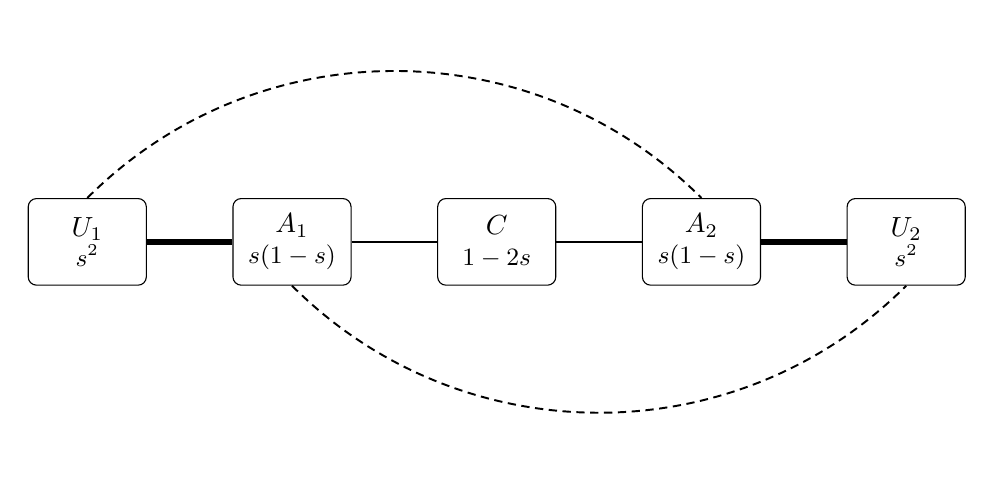
\begin{tikzpicture}[
  part/.style={draw,rounded corners=3pt,minimum width=15mm,minimum height=11mm,align=center,inner sep=2pt},
  joined/.style={line width=0.6pt},
  shared/.style={line width=2.4pt},
  paired/.style={densely dashed,line width=0.7pt}]
 \node[part] (U1) at (0,0) {$U_1$\\[-1pt]\small$s^2$};
 \node[part] (A1) at (2.6,0) {$A_1$\\[-1pt]\small$s(1-s)$};
 \node[part] (C) at (5.2,0) {$C$\\[-1pt]\small$1-2s$};
 \node[part] (A2) at (7.8,0) {$A_2$\\[-1pt]\small$s(1-s)$};
 \node[part] (U2) at (10.4,0) {$U_2$\\[-1pt]\small$s^2$};
 \draw[shared] (U1) -- (A1);
 \draw[joined] (A1) -- (C);
 \draw[joined] (C) -- (A2);
 \draw[shared] (A2) -- (U2);
 \draw[paired] (U1.north) to[out=45,in=135] (A2.north);
 \draw[paired] (A1.south) to[out=-45,in=-135] (U2.south);
\end{tikzpicture}
\caption{The five cliques in the proof of Theorem~\ref{thm:interior}, with their vertex proportions; consecutive cliques are completely joined. The two thick joins are colored injectively with a common palette. The dashed arcs indicate that each edge inside $U_1$ shares its color with a distinct edge inside $A_2$, and each edge inside $U_2$ with a distinct edge inside $A_1$. All other edges receive distinct new colors.}
\label{fig:chain}
\end{figure}

\begin{proof}[Proof of Theorem~\ref{thm:interior}]
Since $\frac12-3s^2+4s^3$ decreases from $1/2$ to $1/4$ on $[0,1/2]$, the parameter $s$ is well defined. Take five disjoint cliques $U_1,A_1,C,A_2,U_2$, in this order, with respective vertex proportions $u,a,c,a,u$, where
\[
 u=s^2,\qquad a=s(1-s),\qquad c=1-2s.
\]
Join consecutive cliques completely and add no other edges between them. Color the two bipartite graphs $U_1$--$A_1$ and $A_2$--$U_2$ injectively with the same set of colors. Also pair each edge inside $U_1$ with a distinct edge inside $A_2$, and each edge inside $U_2$ with a distinct edge inside $A_1$; these pairings are possible because $u\le a$. Use a separate new color for each pair and for each remaining edge. Call the resulting graph $G$.

Every seven-cycle is rainbow. Indeed, if a cycle contains an edge inside $U_1$ and one inside $A_2$, the two paths left after removing these edges each have length at least three. The same holds for edges inside $U_2$ and $A_1$. For an edge of $U_1$--$A_1$ and an edge of $A_2$--$U_2$, the corresponding paths have total length at least $3+3$ or $4+2$, according to the pairing of endpoints. In each case the cycle has at least eight edges, so it cannot be a seven-cycle.

The edge and color counts are
\[
 \begin{aligned}
 e(G)&=\left(\frac{c^2}{2}+a^2+u^2+2ca+2au\right)n^2+O(n)
       =qn^2+O(n),\\
 r(G)&=e(G)-(au+u^2)n^2+O(n)
       =(q-s^3)n^2+O(n).
 \end{aligned}
\]
Here the two bipartite graphs save $au n^2+O(n)$ colors, and the two pairings of internal edges save $u^2n^2+O(n)$ colors. Symmetric rounding, which keeps $|U_1|=|U_2|$ and $|A_1|=|A_2|$, changes these counts by $O(n)$. Since $dq/ds=-6s(1-2s)<0$, decreasing $s$ by $O(1/n)$ if necessary and then deleting excess edges gives the stated upper bound at exactly $\lfloor qn^2\rfloor$ edges.

This upper coefficient is strictly smaller than the one in~\cite{BCM}. Indeed,
\[
 q-\frac14-(q-2s^3)^2=s^3(1-2s)^2(2-s)>0,
\]
and hence
\[
 q-s^3<\frac q2+\frac12\sqrt{q-\frac14}.\qedhere
\]
\end{proof}

\section{Further questions}\label{sec:questions}

\begin{enumerate}
\item Is Theorem~\ref{thm:interior} sharp? That is, for fixed $1/4<q<1/2$ and $s$ as in the theorem, is
\[
 \chi_S(n,\lfloor qn^2\rfloor,C_7)=(q-s^3)n^2+o(n^2)?
\]
The lower bound of Theorem~\ref{thm:density} is strictly smaller at every fixed interior density.

\item If an $n$-vertex graph $G_n$ has $e(G_n)=\lfloor n^2/4\rfloor+1$ and admits a coloring with $n^2/8+o(n^2)$ colors in which every $C_7$ is rainbow, must $G_n$ differ from the disjoint union of two cliques of orders $n/2+o(n)$ by only $o(n^2)$ edge additions and deletions?

The argument of Section~\ref{sec:assembly} gives a partial answer: the normalized degree variance of such graphs tends to zero. Indeed, if $\sigma_n^2\ge v>0$, running that argument with cleaning parameter $\eta=v^2/128$ and reweighting parameter $\lambda=v/16$ in place of $\gamma$ gives $Q(w)\ge1/4+v^2/64$. Theorem~\ref{thm:finite} then forces more than $(1/8+v/70)n^2$ colors for large $n$.

\item Does every $n$-vertex graph with more than $\lfloor n^2/4\rfloor$ edges contain a family of at least $n^2/8-o(n^2)$ edges such that every two lie on a common $C_7$?

A positive answer would strengthen Theorem~\ref{thm:main}, since all edges in such a family must receive different colors. Section~\ref{sec:boundary} constructs such families under its nearly regular hypotheses. The fractional coloring argument in Section~\ref{sec:finite} does not produce such a family in general.

\item Can Theorem~\ref{thm:main} be sharpened to
\[
 \chi_S(n,\lfloor n^2/4\rfloor+1,C_7)=\frac{n^2}{8}+O(n)?
\]
The upper bound already has this error term.

\item Can Theorem~\ref{thm:main} be proved without Szemer\'{e}di's regularity lemma? In particular, can a direct structural argument replace the passage from closed walks to cycles in Section~\ref{sec:cleaning}?

Such an argument could improve the quantitative bounds. Buci\'{c}, Chen and Ma~\cite[Sections~2--4]{BCM} prove their result for longer odd cycles using induction and short-path arguments.
\end{enumerate}

\begin{thebibliography}{99}
\bibitem{Bloom809}
T. F. Bloom, \emph{Erd\H{o}s Problem \#809}, Erd\H{o}s Problems, \url{https://www.erdosproblems.com/809}, accessed 24 September 2026.

\bibitem{BCM}
M. Buci\'{c}, K. Chen and J. Ma, \emph{On a maximal anti-Ramsey conjecture of Burr, Erd\H{o}s, Graham, and S\'{o}s}, arXiv:2603.18952v1 (2026). \url{https://arxiv.org/abs/2603.18952v1}.

\bibitem{BEFGS}
S. A. Burr, P. Erd\H{o}s, P. Frankl, R. L. Graham and V. T. S\'{o}s, \emph{Further results on maximal anti-Ramsey graphs}, in \emph{Graph Theory, Combinatorics, and Applications}, Vol.~1 (Kalamazoo, MI, 1988), Wiley, New York, 1991, pp. 193--206. \url{https://fanchung.ucsd.edu/ron/papers/91_02_anti_ramsey.pdf}.

\bibitem{BEGS}
S. A. Burr, P. Erd\H{o}s, R. L. Graham and V. T. S\'{o}s, \emph{Maximal antiramsey graphs and the strong chromatic number}, J. Graph Theory \textbf{13} (1989), 263--282. \href{https://doi.org/10.1002/jgt.3190130302}{doi:10.1002/jgt.3190130302}.

\bibitem{ESS}
P. Erd\H{o}s, M. Simonovits and V. T. S\'{o}s, \emph{Anti-Ramsey theorems}, in \emph{Infinite and Finite Sets}, Vol.~II (Keszthely, 1973), Colloq. Math. Soc. J\'{a}nos Bolyai \textbf{10}, North-Holland, Amsterdam, 1975, pp. 633--643. \url{https://real.mtak.hu/110457/}.

\bibitem{Hajnal}
A. Hajnal, \emph{A theorem on $k$-saturated graphs}, Canad. J. Math. \textbf{17} (1965), 720--724. \href{https://doi.org/10.4153/CJM-1965-072-1}{doi:10.4153/CJM-1965-072-1}.

\bibitem{KS}
J. Koml\'{o}s and M. Simonovits, \emph{Szemer\'{e}di's regularity lemma and its applications in graph theory}, in \emph{Combinatorics, Paul Erd\H{o}s is Eighty}, Vol.~2, Bolyai Society Mathematical Studies \textbf{2}, J\'{a}nos Bolyai Mathematical Society, Budapest, 1996, pp. 295--352. \url{https://www.renyi.hu/~miki/komsimw.pdf}.

\bibitem{Formalization}
Plasma AI, \emph{Erd\H{o}s Problem 809: rainbow odd cycles}, Lean~4 formalization (2026). \url{https://github.com/plasma-ai/erdos-809}.

\bibitem{SS}
G. N. S\'{a}rk\"{o}zy and S. M. Selkow, \emph{On an anti-Ramsey problem of Burr, Erd\H{o}s, Graham, and T. S\'{o}s}, J. Graph Theory \textbf{52} (2006), 147--156. \href{https://doi.org/10.1002/jgt.20148}{doi:10.1002/jgt.20148}.

\bibitem{Szemeredi}
E. Szemer\'{e}di, \emph{Regular partitions of graphs}, in \emph{Probl\`emes combinatoires et th\'{e}orie des graphes} (Colloq. Internat. CNRS, Orsay, 1976), Colloq. Internat. CNRS 260, CNRS, Paris, 1978, pp. 399--401.

\end{thebibliography}

\end{document}
